% ============================================================
\section{Gaussian Field Placement}
\label{sec:approach}

At the heart of the method is one idea: turn the informal placement goal---sit
near magic states when $T$-heavy, cluster with frequent interaction partners, and
leave room to route---into a scalar field over the lattice whose safe maximum is
the tile we pick. The rest of this section specifies our method. We first define the
influence field cast by a single source and the score that superposes many of them
(\S\ref{sec:fields}), then give the two recipes---\emph{coarse} and \emph{fine}---that
read the field weights off the circuit statistics, and finally describe the greedy
placement-and-routing loop that consumes the score (\S\ref{sec:loop}).

\subsection{Influence Fields and the Placement Score}
\label{sec:fields}

A single \emph{influence field} is an isotropic 2D Gaussian centred at a tile
$(\mu_x,\mu_y)$,
\begin{equation}
g(x,y) \;=\; w\,\exp\!\Big(\!-\frac{(x-\mu_x)^2+(y-\mu_y)^2}{2\sigma^2}\Big),
\label{eq:gauss}
\end{equation}
with a non-negative weight $w$. A field is either \emph{attractive}, contributing
$g(x,y)$, or \emph{repulsive}, contributing the valley
$\max\!\big(w-g(x,y),\,0\big)$, which is near zero at the centre and rises to $w$
far away; attractive sources thus pull a qubit in, repulsive sources push it out.
A single width $\sigma$---the same on both axes and independent of the grid
size---sets the reach of every field: a larger $\sigma$ spreads a source's
influence over more tiles, a smaller one keeps it local. We use one tuned value of
$\sigma$ for all fields (Section~\ref{sec:eval}). To bound work, each field is
evaluated only within a bounded window around its centre, where its contribution
is non-negligible, and takes the field's limiting value beyond it---zero if attractive, $w$ if repulsive.

When placing a qubit $q$, the score at a free tile $v$ superposes four families of
fields,
\begin{equation}
S(v)\!=\!\!\!
   \underbrace{\sum_{m\in V_{\mathrm m}}\! g^{\mathrm{mag}}_m(v)}_{\text{magic-state pull/push}}
 +\!\underbrace{\sum_{p\in P(q)}\! g^{\mathrm{cnot}}_p(v)}_{\text{partner clustering}}
 + \underbrace{\sum_{u\in \M}\! g^{\mathrm{rep}}_u(v)}_{\text{spread-out}}
 +\!\underbrace{b(v)}_{\text{centering}}\!\!,
\label{eq:score}
\end{equation}
where $P(q)$ is the set of $q$'s interaction partners (the qubits sharing a gate
with $q$) and the repulsion sum ranges over the qubits already committed by the
partial mapping $\M$ (Definition~\ref{def:mapping}). The \emph{magic-state}
term puts one Gaussian on every magic tile $m\in V_{\mathrm m}$, whose sign and
weight encode $q$'s $T$ demand: a $T$-heavy qubit makes them attractive and is
drawn toward magic states, whereas a $T$-light qubit makes them repulsive,
clearing those neighbourhoods for the qubits that need them. The
\emph{partner} term puts an attractive Gaussian on the tile of each
already-mapped partner $p\in P(q)$, pulling strongly coupled qubits together so
their future surgeries traverse short corridors. The \emph{repulsion} term puts a
repulsive Gaussian on every already-placed qubit $u\in\M$, discouraging
overcrowding. Finally $b(v)$ is a single attractive
Gaussian at the grid centre that keeps the overall mapping compact; in the regime
where magic states sit on the lattice boundary we subtract a tuned constant from every border tile, penalising boundary placements that obstruct magic state tiles.
Figure~\ref{fig:fields} shows the four families and their superposition. Crucially,
only partners and patches \emph{already committed} contribute, so the field seen by a qubit depends on the placement order---which we exploit in
Section~\ref{sec:loop}.

% ---- FIGURE: influence-field decomposition (single column) ----
\begin{figure}[t]
    \centering
    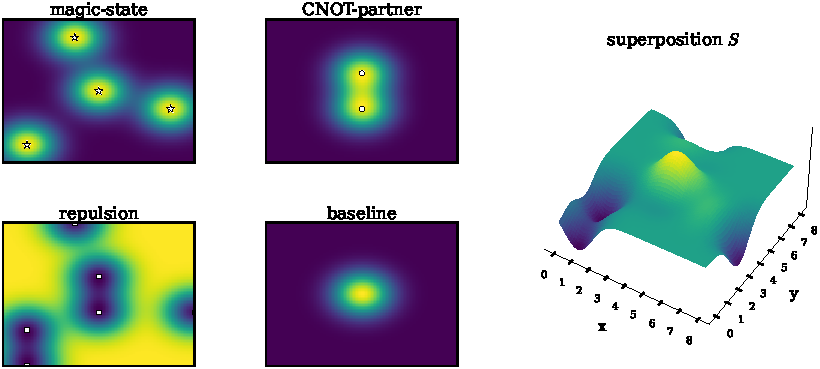
\includegraphics[width=\linewidth]{figures/gaussian_fields.pdf}
    \caption{Decomposition of the Gaussian fields for one qubit: the
    magic-state, CNOT-partner, repulsion, and baseline field families (heatmaps,
    left) and their superposition $S$ as a surface over the lattice (right).
    Markers denote the magic tiles ($\star$), the qubit's interaction partners
    ($\circ$), and already-placed patches ($\square$); the red marker on $S$ is
    its safe maximum.}
    \label{fig:fields}
    \vspace{-0.5cm}
\end{figure}


\subsection{Coarse and Fine Weighting}

The two variants differ only in how each field's weight $w$ and its
attractive/repulsive sign are read off the circuit statistics. Both use a small
set of non-negative tuned constants---\textsc{magic-high}, \textsc{magic-low} for
the magic fields and \textsc{cnot-high} for the partner fields---whose values are
fixed per regime by the sweeps of Section~\ref{sec:eval} and listed in the
repository~\cite{ftqc}.

The \emph{coarse} variant makes discrete decisions from a qubit's $T$-count $t(q)$
and its largest single-partner CNOT count $c_{\max}(q)=\max_{p}c(q,p)$: the qubit
is \emph{$T$-bound} when $t(q)>c_{\max}(q)$ and \emph{partner-driven} otherwise.
Its magic-field weight switches on only for qubits whose $T$ demand is more than
one standard deviation from the mean,
\begin{equation*}
w^{\mathrm{mag}}_q \;=\;
\begin{cases}
\textsc{magic-high}, & |t(q)-\bar t|>\sigma_t,\\[2pt]
0, & \text{otherwise,}
\end{cases}
\end{equation*}
the field being attractive if $t(q)>c_{\max}(q)$ and repulsive if
$t(q)\le c_{\max}(q)$. In the partner-driven regime it also adds an attractive
CNOT field at every mapped partner $p$ with above-average interaction
($c(q,p)\ge\bar c$), and triples the pull toward the single dominant partner
$p^{\star}=\arg\max_p c(q,p)$,
\begin{equation*}
w^{\mathrm{cnot}}_{p} \;=\;
\begin{cases}
3\,\textsc{cnot-high}, & p=p^{\star},\\[2pt]
\textsc{cnot-high}, & \text{otherwise.}
\end{cases}
\end{equation*}

The \emph{fine} variant replaces the thresholds with linear interpolation, writing
$\mathrm{lerp}(a,b,s)=a+s\,(b-a)$ for $s\in[0,1]$. For the magic fields,
\begin{equation*}
w^{\mathrm{mag}}_q =\!
\begin{cases}
\textsc{magic-high}, & \hspace{-40pt} |t(q)-\bar t|>\sigma_t,\\[2pt]
\mathrm{lerp}\!\big(\textsc{magic-low},\textsc{magic-high},\tfrac{|t(q)-\bar t|}{\sigma_t}\big), & \hspace{5pt} \text{else},
\end{cases}
\end{equation*}
attractive when $t(q)>\bar t$ and repulsive when $t(q)<\bar t$; the CNOT fields are
weighted analogously from the per-pair count $c(q,p)$ relative to $\bar c$ and
$\sigma_c$. Fine thus reacts smoothly to how far a qubit deviates from the
circuit's average resource profile, while coarse commits to a hard on/off split.

\subsection{Placement-and-Routing Loop}
\label{sec:loop}

Placement is greedy and proceeds in a single pass. We first rank qubits by
\emph{interaction importance}---a qubit's $T$-count plus its largest single-partner
CNOT count---and commit the most important first, so the mapping forms around the
qubits that constrain it most while the lattice is still empty. Because a qubit's
partner fields act only on partners that are already placed, the visiting order
matters on sparse circuits: when the CNOT interaction graph has density below a
threshold $\tau$ ($0.7$ by default) we expand placement in \emph{CNOT-BFS} order,
starting from the highest-importance qubits and visiting each interaction
neighbourhood breadth-first, heaviest partner first, so every qubit finds its
strongest partner already in place; on dense graphs, which offer no such locality,
we keep the plain importance order. For each qubit we evaluate the score $S$ of
\eqref{eq:score} on every free tile, sort the tiles by decreasing $S$, and commit
the first that doesn't violate safe passage
(Definition~\ref{def:safepassage}), adding a repulsion field there; if no tile
passes, placement reports failure.
Algorithm~\ref{alg:main} summarises the loop and Figure~\ref{fig:frames} shows the potential-field variation as
the mapping grows.

% ---- ALGORITHM: Gaussian field placement ----
\begin{algorithm}[t]
\caption{Gaussian field placement}
\label{alg:main}
\begin{algorithmic}[1]
    \Require Circuit $\C$, architecture $\A$ with magic tiles $V_{\mathrm m}$
    \Ensure Safe-passage mapping $\M$
    \If{CNOT-graph density $<\tau$}
        \State order $\Q_L$ by CNOT-BFS
    \Else
        \State order $\Q_L$ by interaction importance
    \EndIf
    \State $\M \gets \emptyset$;\; add baseline field; add magic fields
    \For{$q$ in order}
        \State build magic/CNOT field weights
        \State $S(v)\gets$ superpose fields over each free tile $v$
        \For{$v$ in tiles sorted by $S(v)$ descending}
            \If{\Call{SafePassage}{$v,q,\M$}}
                \State $\M(q)\gets v$;\; add repulsion field at $v$;\; \textbf{break}
            \EndIf
        \EndFor
        \If{no tile committed} \State \textbf{fail} (no routable placement) \EndIf
    \EndFor
    \State \Return $\M$
\end{algorithmic}
\end{algorithm}


The resulting mapping is handed to the router, which produces a routing
$\Rout$ (Definition~\ref{def:routing}). Our \emph{packing} router schedules as many
vertex-disjoint corridors per step $P_i$ as it can, prioritising gates that are
critical to the downstream schedule, and serves $T$ gates with a dedicated
strategy that reserves a corridor to the nearest free magic-state tile; a simpler
\emph{naive-critical} shortest-path router is also available. Because the mapping already
satisfies safe passage (Definition~\ref{def:safepassage}), every gate stays
reachable and the router never deadlocks---its only job is to keep $|\Rout|$ small
by packing each step densely.

The two routers differ in how they fill each step. The
\emph{packing} router proposes a few
candidate corridors for every waiting gate and then greedily commits a 
maximal mutually disjoint subset, taking gates
in order of \emph{downstream criticality} (how many of the next few layers depend
on each gate's qubits) and deferring whatever does not fit to the following step.
The \emph{naive-critical} router is the lightweight alternative: it lays down a
single shortest path per gate, visits gates in the same criticality order, and
simply defers any gate whose path would collide with one already placed.
It is cheaper but packs each step less densely, so it generally
uses more routing steps than packing. The full routers are described in the
artifact~\cite{ftqc}.

% ---- FIGURE: mapping-formation frames (single column) ----
\begin{figure}[t]
    \centering
    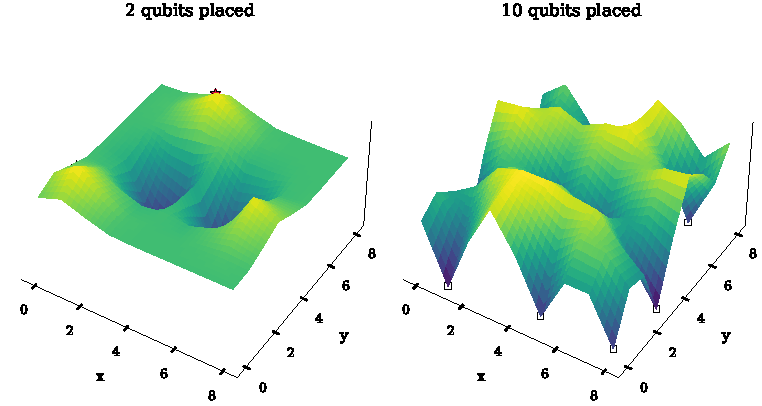
\includegraphics[width=\linewidth]{figures/gaussian_frames.pdf}
    \caption{Formation of a Gaussian-field mapping: the (per-panel normalised)
    score surface $S$ after the indicated number of qubits are committed. White
    squares are committed patches, red stars magic tiles; repulsion carves a well
    at each patch, spacing qubits apart.}
    \label{fig:frames}
    \vspace{-0.5cm}
\end{figure}


\begin{remark}
Evaluating the field for one qubit costs
$O(|V|\cdot(|V_{\mathrm m}|+|P(q)|+|\Q_L|))$, and with the lattice sized as
$\Theta(|\Q_L|+|V_{\mathrm m}|)$ tiles the whole placement is low-order
polynomial in the qubit count.
\end{remark}
